\documentclass[conference]{IEEEtran}
\IEEEoverridecommandlockouts
\usepackage{cite}
\usepackage{amsmath,amssymb,amsfonts}
\usepackage{algorithmic}
\usepackage{graphicx}
\usepackage{textcomp}
\usepackage{xcolor}
\usepackage{float}
\usepackage{hyperref}
\usepackage{listings}
\usepackage{pgfplots}
\usepackage{booktabs}
\usepackage{tikz} % Required for TikZ drawings
\pgfplotsset{compat=1.18}
\def\BibTeX{{\rm B\kern-.05em{\sc i\kern-.025em b}\kern-.08em
    T\kern-.1667em\lower.7ex\hbox{E}\kern-.125emX}}
\lstdefinestyle{mystyle}{
    basicstyle=\ttfamily\footnotesize,
    breakatwhitespace=false,         
    breaklines=true,                 
    captionpos=b,                    
    keepspaces=true,                                                       
    showspaces=false,                
    showstringspaces=false,
    showtabs=false,                  
    tabsize=2,
    frame=single,
    rulecolor=\color{black}
}
\lstset{style=mystyle}
\providecommand{\tabularnewline}{\\}
\floatstyle{ruled}
\newfloat{algorithm}{tbp}{loa}
\providecommand{\algorithmname}{Algorithm}
\floatname{algorithm}{\protect\algorithmname}
\usetikzlibrary{calc}



\title{Benchmarking Sorting Algorithms: Selection, Merge and Heap Sort in C}
\author{\IEEEauthorblockN{Daniel Marin} \IEEEauthorblockA{\textit{Department of Computer Science}} \\ \textit{Texas Tech University} \\ San Jose, Costa Rica \\ danimari@ttu.edu}

\begin{document}
\maketitle
\begin{abstract}
The purpose of this paper is to provide an analysis on the efficiency of various sorting algorithms previously studied: Heap Sort, Merge Sort and Selection Sort. The analysis looks to quantify and verify if the theoritical differences in efficiency match real life; by creating an implementation in real life and contrasting the performance. Each algorithm was tested on arrays of randomly chosen integers of sizes: 50.000, 100.000, 150.000, and 200.000. The execution time of each run was measured, and analyzed to identify and look for discrepencies between the theoretical time complexities of each algorithm and their practical performance. 
\end{abstract}

\begin{IEEEkeywords}
Heap Sort, Merge Sort, Selection Sort, Time Complexities, Practical Implementation
\end{IEEEkeywords}

\section{Introduction}
\IEEEPARstart{The}{Sorting} Algorithms are fundamental in the area of computer science, they are the backbone of many of the algorithms, applications and systems we humans use on a daily basis. They play a critical role in making systems faster and more efficient. Thus, the efficiency of a sorting algorithm is a critical factor in determining the performance of various computational tasks that rely on them. The objective of this project is to implement and compare the efficiency of some of those sorting algorithms: Selection Sort, Merge Sort, and Heap Sort.

The primary goals of this paper is to:
\begin{itemize}
    \item Verify that the theoretical differences in efficiency match the implemented performances
    \item Analyze the execution times of these algorithms in arrays of sizes: 50.000, 100.000, 150.000, and 200.000
    \item Draw meaningful conclusions about their efficiency and performance characteristics
\end{itemize}

Each algorithm that will be analyzed has a different method into sorting a list, with their respective time complexity. The time complexities, which are a measure of the algorithm's execution efficiency, depend on the size of the input data. Selection Sort has a time complexity of $\Theta(n^{2})$, but a fairly simple implementation making it suitable for small datasets and simple systems. Merge and Heap Sort have a time complexity of $\Theta(nlogn)$ making them more efficient when dealing with large datasets, but require a complex implementation.

The environment of the system in which the project is being developed is the following: program will be developed in C, algorithms will sort arrays of the sizes stated above, and the development of tables and graphs will be done in LaTeX. 

With the tests and results we look to observe the scalability of each algorithm as the size of the input increases, and compare those results by analyzing the shape of the execution times curves to identify the trends and patterns. Specificially, we look to visualize that the time complexies of each algorithm match their execution times. So, we expect the curve of $\Theta(n^{2})$ to be exhibited in the graphs related to the selection sort algorithm, while the curve of $\Theta(nlogn)$ to be present in the graphs of the other two algorithms. The results of this paper will provide the valuable insights into the reality of these algorithms in application. 

\section{Methodology}
This section looks to outline the procedures followed to conduct the experiments and collect the necessary data for evaluating the performance of the implemented sorting algorithms. This section provides information about the programming environment, data generation process, execution of experiments, and the algorithms in it. For this paper, three algorithms where used: Selection Sort, Merge Sort and Heap Sort\footnote{The program expected Merge Sort implementation to use \texttt{mergesort} and Heap Sort's to use \texttt{heapsort} as the names of the functions, but do to an issues with the \texttt{stdlib.h} library the names where changed to \texttt{merge\_sort} and \texttt{heap\_sort}}.
\subsection{Selection Sort}
Selection sort is a simple algorithm that repeatedly finds the minimum element from the unsorted part of the array and puts it at the beginning of that part. This process continues until the entire array has been sorted. The implementation is as follows: 
\begin{lstlisting}[language=C]
void selection_sort(int A[], int n) {
    for (int i = 0; i < n - 1; i++) {
        int minInd = i;
        for (int j = i + 1; j < n; j++)
            if (A[j] < A[minInd])
                minInd = j;
        swap(&A[minInd], &A[i]);
    }
}   
\end{lstlisting}
\subsection{Merge Sort}
Merge Sort is a divide-and-conquer algorithm that divides the array into 'equal' halves, recursively sorts the two halves, and then merges them to produce a single sorted array. The main issue this algorithm poses is it's space complexity of $\Theta(n)$ making it unsuitable for big data sets. 

The merge sort is implemented using three functions:
\begin{itemize}
    \item \texttt{merge}: this function merges two sorted subarrays into a single sorted array. The implementation is as follows:
    \begin{lstlisting}[language=C]
void merge(int A[], int beg, int mid, int end) {
    int i = beg, j = mid + 1, index = 0;
    int size = end - beg + 1;
    int* temp = (int*)malloc(size * sizeof(int));
    if (!temp) {
        perror("malloc failed");
        exit(EXIT_FAILURE);
    }
    while (i <= mid && j <= end) {
        if (A[i] <= A[j]) {
            temp[index++] = A[i++];
        } else {
            temp[index++] = A[j++];
        }
    }
    while (i <= mid) {
        temp[index++] = A[i++];
    }
    while (j <= end) {
        temp[index++] = A[j++];
    }
    for (i = 0; i < size; i++) {
        A[beg + i] = temp[i];
    }
    free(temp); 
}
    \end{lstlisting}
    \item \texttt{merge\_sort\_rec}: this function is in charge of the recursive behavior of the Merge Sort algorithm of dividing the array into halves. The implementation is as follows:
    \begin{lstlisting}[language=C]
void merge_sort_rec(int A[], int beg, int end) {
    if (beg < end) {
        int mid = (beg + end) / 2;
        merge_sort_rec(A, beg, mid);
        merge_sort_rec(A, mid + 1, end);
        merge(A, beg, mid, end);
    }
}
    \end{lstlisting}
    \item \texttt{merge\_sort}: this is the main function of the algorithm that calls the recursive version. The implementation is as follows:
    \begin{lstlisting}[language=C]
void merge_sort(int A[], int n) {
    merge_sort_rec(A, 0, n - 1);
}
    \end{lstlisting}
\end{itemize}
The behavior of this algorithm is encapsulated and implemented with the use of the aforementioned functions. 
\subsection{Heap Sort}
Heap Sort is a comparison-based sorting algorithm that usesa binary heap data structure to sort the elemenents of the array. In practice Heap Sort, builds a max heap from the array. Then, it repeatedly extracts the maximum element form the heap (the root) and rebuilds the heap, will not considering the extracted element.

The functions used to implement the behavior of this algorithm are the following:
\begin{itemize}
    \item \texttt{heapify}: this function is used to build a max heap from the array. The implementation is as follows:
    \begin{lstlisting}[language=C]
void heapify(int A[], int n, int i) {
    int largest = i;
    int left = 2 * i + 1;
    int right = 2 * i + 2;
    if (left < n && A[left] > A[largest])
        largest = left;
    if (right < n && A[right] > A[largest])
        largest = right;

    // Swap and continue heapifying if root is not largest
    if (largest != i) {
        swap(&A[i], &A[largest]);
        heapify(A, n, largest);
    }
}   
    \end{lstlisting}
    \item \texttt{swap}: this function is in charge of swapping elements in the array. The implementation is as follows:
    \begin{lstlisting}[language=C]
        void swap(int *a, int *b) {
            int temp = *a;
            *a = *b;
            *b = temp;
            }       
    \end{lstlisting}
    \item \texttt{heap\_sort}: this is the main function that builds the max heap, repeatedly extracts the maximum element and rebuilds the heap until the array is sorted. The implementation is as follows:
    \begin{lstlisting}[language=C]
void heap_sort(int A[], int n) {
    // Heapify Original Array
    for (int i = n / 2 - 1; i >= 0; i--)
        heapify(A, n, i);
    // Heap Sort
    for (int i = n - 1; i >= 0; i--) {
        swap(&A[0], &A[i]);
        heapify(A, i, 0);
    }
}    
    \end{lstlisting}
\end{itemize}

\subsection{Environmental Setup}
The experiments where conducted using a C programming environment developed in VSCode on a computer system. The programming environment included the use of C libraries that provided basic functionality for the program to be meaningful. The experiments where performed on an operating system with no other significant processes running in the background to ensure consistent results.

The system specifications for the computer system utilized in the development of this computer are as follows:
\begin{itemize}
    \item Operating System: [Windows 11 Home: 64 Bit]
    \item Processor: [Intel Core i5-10400F, 2.90 GHz (6 cores)]
    \item RAM: [32 GB]
    \item Storage: [SSD, 1TB]
\end{itemize}

\subsection{Test Formats}
The tests performed where as follows: an array of size ranging from 50.000 to 200.000 in 50.000 increments was filled with random numbers using the rand() function from the stdlib.h library, then the sorting algorithm was called using the following function that was in charge of measuring the execution time of the algorithm taking place:
\begin{lstlisting}[language=C]
double measureSortTime(SortFunction func, int arr[], int n) {
    clock_t start, end;
    start = clock();
    func(arr, n);
    end = clock();
    check_unsorted(arr, n);
    return ((double)(end - start)) / CLOCKS_PER_SEC;
}
\end{lstlisting}
Each sorting algorithm was measured 3 times per size, until all of the desired results where measured. 
\subsection{Limitations} 
The experiments are designed to provide meaningful insights into the performance and where developed to be run in any computer with access to a C compiler, we must take into consideration that there are some limitations out of our control such as: system resource constraints, potential biases introduced by the standard C libraries, and the overall capabilities of the hardware of the computer system. These limitations will influence the end results of this paper, still the behavior of the algorithms should still provide the insight we are looking to demonstrate.

\section{Results}
In this section we present the results of the experiments conducted to analyze the performance of the three sorting algorithms, while handling arrays of varying sizes (50.000 to 200.000 in intervals of 50.000).
\begin{table}[H]
    \caption{Time of Execution of Algorithms\label{tab:tiempos}}
    \centering{}
    \begin{tabular}{lrrrrr}
        \toprule
        &  & \multicolumn{3}{c}{Time (s)}\tabularnewline
        \cmidrule{1-6}
        &  & \multicolumn{4}{c}{Execution Time}\tabularnewline
        \cmidrule{3-5}
        Algorithm & Size (k) & 1 & 2 & 3 & Mean\tabularnewline
        \midrule
        Selection & 50000 & 2.4970 & 2.4900 & 2.4650 & 2.4840 \tabularnewline
        \tabularnewline
        & 100000 & 9.8030 & 9.7680 & 9.7950 & 9.7887\tabularnewline
        \tabularnewline
        & 150000 & 22.005 & 21.974 & 21.995 & 21.9913\tabularnewline
        \tabularnewline
        & 200000 & 39.083 & 39.114 & 39.059 & 39.0853\tabularnewline
        \midrule
        Merge & 50000 & 0.0012 & 0.0012 & 0.0011 & 0.0012\tabularnewline
        \tabularnewline
        & 100000 & 0.0160 & 0.0210 & 0.0220 & 0.0197\tabularnewline
        \tabularnewline
        & 150000 & 0.0340 & 0.0360 & 0.0330 & 0.0343\tabularnewline
        \tabularnewline
        & 200000 & 0.0410 & 0.0480 & 0.0470 & 0.0453\tabularnewline
        \midrule
        Heap & 50000 & 0.0011 & 0.0015 & 0.0017 & 0.0014\tabularnewline
        \tabularnewline
        & 100000 & 0.0230 & 0.0120 & 0.0220 & 0.0190\tabularnewline
        \tabularnewline
        & 150000 & 0.0350 & 0.0330 & 0.0470 & 0.0383\tabularnewline
        \tabularnewline
        & 200000 & 0.0470 & 0.0490 & 0.0540 & 0.0500\tabularnewline
        \bottomrule
    \end{tabular}
\end{table}
\indent The mean execution times are plotted in figure~\ref{fig:lin1}, \ref{fig:lin2}, and \ref{fig:lin3}. This figure represents the graph of the data plotted in Table~\ref{tab:tiempos}. For comparison, purposes the curves are shown together in the same graph in Figure~\ref{fig:log}. Similarly, this figure represents the trends of each sorting algorithm and the average - execution time of each array size, all on the same graph of the data in Table~\ref{tab:tiempos}.
\begin{figure}[H]
    \centering
    \begin{tikzpicture}
        \begin{axis}[name=plot1,
            width=0.9\columnwidth,
            xtick={0,50,100,150,200},
            ylabel=Time (s),
            xlabel=Array Size (k$\times10^{3}$),
            title=\textbf{Selection Sort}]
            \addplot coordinates {(50,2.484) (100,9.7887) (150,21.9913) (200,39.693)};
        \end{axis}
    \end{tikzpicture}
    \caption{Average execution time of Selection Sort algorithms \label{fig:lin1}}
\end{figure}
\begin{figure}[H]
    \centering
    \begin{tikzpicture}
        \begin{axis}[name=plot1,
            width=0.9\columnwidth,
            xtick={0,50,100,150,200},
            ylabel=Time (s),
            xlabel=Array Size (k$\times10^{3}$),
            title=\textbf{Merge Sort}]
            \addplot coordinates {(50,0.0012) (100,0.0197) (150,0.0343) (200,0.0453)};
        \end{axis}
    \end{tikzpicture}
    \caption{Average execution time of Merge Sort algorithms \label{fig:lin2}}
\end{figure}
\begin{figure}[H]
    \centering
    \begin{tikzpicture}
        \begin{axis}[name=plot1,
            width=0.9\columnwidth,
            xtick={0,50,100,150,200},
            ylabel=Time (s),
            xlabel=Array Size (k$\times10^{3}$),
            title=\textbf{Heap Sort}]
            \addplot coordinates {(50,0.0014) (100,0.0190) (150,0.0383) (200,0.0500)};
        \end{axis}
    \end{tikzpicture}
    \caption{Average execution time of Heap Sort algorithms \label{fig:lin3}}
\end{figure}

\begin{figure}[H]
    \begin{centering}
    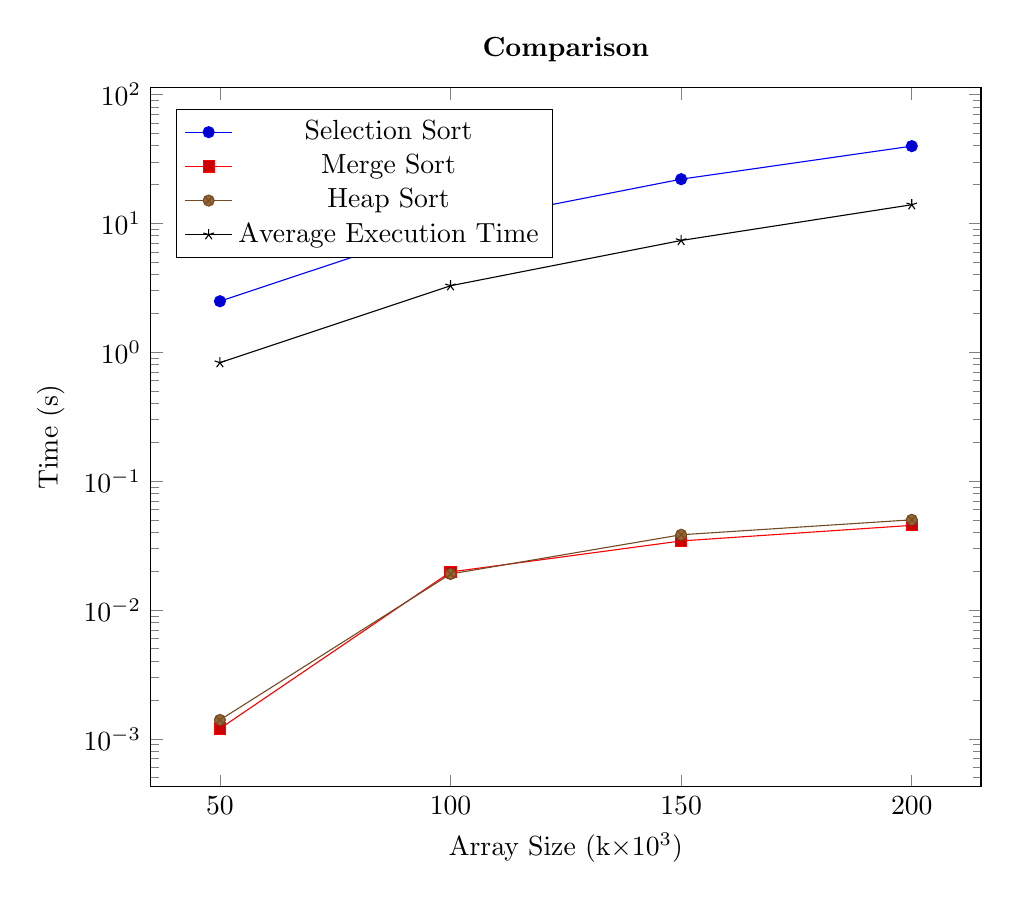
\begin{tikzpicture}
        \begin{semilogyaxis}[
            width=\columnwidth,
            xtick={0,50,...,200},
            xlabel=Array Size (k$\times10^{3}$),
            ylabel=Time (s),
            legend pos=north west,
            title=\textbf{Comparison}]
        \addplot coordinates{(50,2.484) (100,9.7887) (150,21.9913) (200,39.693)};
        \addplot coordinates{(50,0.0012) (100,0.0197) (150,0.0343) (200,0.0453)};
        \addplot coordinates{(50,0.0014) (100,0.0190) (150,0.0383) (200,0.0500)};
        \addplot coordinates{(50,0.8289) (100,3.2758) (150,7.3546) (200,13.9294)};
        \legend{Selection Sort,Merge Sort,Heap Sort, Average Execution Time}
        \end{semilogyaxis}
    \end{tikzpicture}
    \par\end{centering}
    
    \caption{Comparing mean execution times of sorting algorithms.\label{fig:log}}
\end{figure}
\subsection{Analysis of Sorting Algorithms: Selection Sort}
Selection Sort is a simple algorithm, it looks to divide an input array into two parts: a sorted subarray and an unsorted subarray. The algorithm repeatedly selects the smallest (ascending) element from the unsorted subarray and moves it to the end of the sorted subarray. This process continues until the entire array is sorted. 

The time complexity of the Selection Sort is $\Theta(n^2)$, where $n$ is the size of the array. This is because it has $n-1$ comparison in the first iteration, $n-2$ comparisons in the second, and so on, resulting in a total of $\frac{n(n-1)}{2}$ in total. Additionaly, it may need to perform swap operations. 

Due to its simplicity, Selection Sort is not suitable for large datasets due to its quadratic time complexity. However, it might find use when studying algorithms or for sorting small datasets.

In this experiment, we implemented Selection Sort in C and tested its performance by measuring the execution times on arrays ranging from 50,000 and 200,000 elements. The execution times were measured, and the results were analyzed to assess the algorithm's real efficiency. The mean execution times of Selection Sort for different array sizes are as follows:
\begin{itemize}
    \item Array size 50,000 elements, has a 2.474 seconds mean execution time.
    \item Array size 100,000 elements, has a 9.7887 seconds mean execution time.
    \item Array size 150,000 elements, has a 21.9913 seconds mean execution time.
    \item Array size 200,000 elements, has a 39.693 seconds mean execution time.
\end{itemize}

These results confirm that the execution time of Selection Sort grows quadratically as array size increases, which is consistnet with its $\Theta(n^2)$ time complexity. 
\subsection{Analysis of Sorting Algorithms: Merge Sort}
Merge Sort as stated above is a divide-and-conquer algorithm that divides the input array into two halves, recursively sorts the two halves, and merges them to produce a single sorted array. 

The time complexity of Merge Sort is $\Theta(nlogn)$, where $n$ is the size of the array. This makes it more efficient than Selection Sort. 

In this experiment, we implemented Merge Sort in C and tested its performance by measuring the execution times on arrays ranging from 50,000 and 200,000 elements. The execution times were measured, and the results were analyzed to assess the algorithm's real efficiency. The mean execution times of Merge Sort for different array sizes are as follows:
\begin{itemize}
    \item Array size 50,000 elements, has a 0.0012 seconds mean execution time.
    \item Array size 100,000 elements, has a 0.0197 seconds mean execution time.
    \item Array size 150,000 elements, has a 0.0343 seconds mean execution time.
    \item Array size 200,000 elements, has a 0.0453 seconds mean execution time.
\end{itemize}

These results confirm that the execution time of Merge Sort grows logarithmically with size of the input array, consistent with its time complexity of $\Theta(nlogn)$. 

\subsection{Analysis of Sorting Algorithms: Heap Sort}
Heap Sort is a comparison-based sorting algorithm that uses a binary heap data structure to build a partially sorted heap. It then repeatedly extracts the maximum (for a max-heap) element and places it at the end of the sorted array.

The time complexity of Heap Sort is $\Theta(nlogn)$, where $n$ is the size of the array. Yet, it isn't as efficient as Merge Sort in most cases due to the overhead of heapifying after every step. 

In this experiment, we implemented Heap Sort in C and tested its performance by measuring the execution times on arrays ranging from 50,000 and 200,000 elements. The execution times were measured, and the results were analyzed to assess the algorithm's real efficiency. The mean execution times of Heap Sort for different array sizes are as follows:
\begin{itemize}
    \item Array size 50,000 elements, has a 0.0014 seconds mean execution time.
    \item Array size 100,000 elements, has a 0.0190 seconds mean execution time.
    \item Array size 150,000 elements, has a 0.0383 seconds mean execution time.
    \item Array size 200,000 elements, has a 0.0500 seconds mean execution time.
\end{itemize}

These results confirm that the execution time of Heap Sort grows logarithmically with size of the input array, consistent with its time complexity of $\Theta(nlogn)$; and that it performs slightly worse than Merge Sort. 

\subsection{Comparisons and Conclusion}
\begin{itemize}
    \item Merge Sort: With it't time complexity $\Theta(nlogn)$ and consistent performance across different input sizes, is the best performing sorting algorithm for large data sets.
    \item Heap Sort: Although theoretically efficient, Heap Sort seems to fall short of the performance of the Merge Sort algorithm but compensates by having a space complexity of $\Theta(1)$ compared to the Merge Sort's space complexity of $\Theta(n)$.
    \item Selection Sort: This algorithm, with its time complexity of $\Theta(n^2)$, are not suitable for efficiently sorting large data sets and are outperformed by Merge and Heap sort by a large margin. 
\end{itemize}
In conclusion, Merge Sort and Heap Sort are the recommended sorting algorithms for large data sets and overall efficiency. Both having time complexities of $\Theta(n^2)$, making them efficient for all types of input sizes, and they can also use any type of data that may be compared. 

\begin{thebibliography}{1}

\bibitem{website}
Programiz, \emph{Heap sort}. Available: \url{https://www.programiz.com/dsa/heap-sort}. Accessed: 2024-10-29.

\bibitem{website}
Programiz, \emph{Merge Sort}. Available: \url{https://www.programiz.com/dsa/heap-sort}. Accessed: 2024-10-29.

\bibitem{website}
Programiz, \emph{Selection Sort}. Available: \url{https://www.programiz.com/dsa/heap-sort}. Accessed: 2024-10-29.
\end{thebibliography}
\end{document}